\documentclass{article}
\usepackage{amsmath}
\usepackage{amssymb}
\usepackage{graphicx}
\usepackage{hyperref}
\usepackage[version=4]{mhchem}


\begin{document}
(AMC) A triangle has angles of \(30^{\circ}\) and \(45^{\circ}\). If the side opposite the \(45^{\circ}\) angle has length 8 , then the side opposite the \(30^{\circ}\) angle has length\\
(A) 4\\
(B) \(4 \sqrt{2}\)\\
(C) \(4 \sqrt{3}\)\\
(D) \(4 \sqrt{6}\)\\
(E) 6

Solution: (B).\\
Let \(s\) denote the length of the side we want to figure out (see figure to the right). The altitude to the longest side, opposite the \(30^{\circ}\) angle, has length \(\frac{8}{2}=4\) and is also one leg of an isosceles right triangle with hypotenuse \(s\), which therefore has length\\
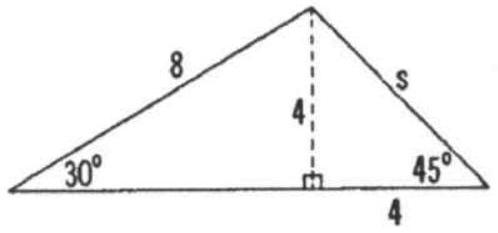
\includegraphics[width=\textwidth]{images/075(1).jpg} \(4 \sqrt{2}\).


\end{document}
